\documentclass[12pt,a4pape, fullpage]{article}
\usepackage[
margin=1.5cm,
includefoot,
footskip=30pt,
]{geometry}
\usepackage[utf8]{inputenc}
%\usepackage[T1]{fontenc}
\usepackage{amsmath}
\usepackage{amsfonts}
\usepackage{amssymb}
\usepackage{graphicx}
\usepackage{comment}
\usepackage{natbib}
\usepackage{lineno}

\bibliographystyle{evolution.bst}

\newcommand{\norm}[1]{\left\lVert#1\right\rVert}
\newcommand{\normsq}[1]{\left\lVert#1\right\rVert^2}


\newcommand{\MX}{\mathbf{X}} %uncentered data
\newcommand{\MC}{\mathbf{C}} %centering
\newcommand{\MY}{\mathbf{Y}} %centered data
\newcommand{\MF}{\mathbf{F}_2} %F2-distance matrix
\newcommand{\MFT}{\mathbf{F}_3} %F3-distance matrix
\newcommand{\MP}{\mathbf{P}} % PCs
\newcommand{\ML}{\mathbf{L}} % loadings
\newcommand{\MK}{\mathbf{K}} % Kernel
\newcommand{\MSINGULAR}{\mathbf{\Sigma}} % Singular values matrix
\newcommand{\MEIGEN}{\mathbf{\Lambda}} % Eigenvalue matrix


\newcommand{\MEAN}{\boldsymbol{\mu}} % Kernel
\begin{document}
\section{Introduction}
About 15\% of genetic variation in humans can be explained by population structure \cite{lewontin1972, barbujani1997, rosenberg2003}, but the information contained in these 15\% is sufficient to study the genetic diversity and history in great detail \cite{cavalli-sforza1994, edwards2003}. For some data sets it is possible to predict an individuals origin at a resolution of a few hundred kilometers \cite{novembre2008, leslie2015}, and direct-to-consumer-genetics companies are using this variation to analyze the genetic data of millions of customers.

However, population genetic models that adequately capture the heterogeneity in human genetic diversity remain a challenge. 
It is also apparent that human genetic variation is largely distributed in gradients.
In Lewontin's pioneering analysis, he found that less than half (6\%), of that variation could be attributed to the continental-scale groups. Later studies on genome-wide data show 

although some discontinuities, often associated with obstacles to migration such as mountain ranges or oceans, exist \cite{serre2004, ramachandran2005, rosenberg2007, peter2020}. 

One related question is how discrete human populations are. While human genetic differentiation generally increases with geographic distance \cite{ramachandran2005, rosenberg2007}, this increase is not uniform. Obstacles to migration,  such as oceans, mountains or deserts do frequently cause discontinuities in population structure \cite{peter2020a}. Thus, while barriers to gene flow rarely are absolute, segregation policies by (perceived) ethnic or racial ancestry frequently cause local small-scale population differentiation that persist to the present day.

As a consequence, tools such as Principal Component Analysis (PCA) are frequently used to visualize or model human population structure \citep{cavalli-sforza1964, cavalli-sforza1994}. Informally, PCA aims to extract the axes of largest variation in a data set; for population genetic data sets of e.g. SNPs, these axes typically reflect population structure and need to be taken into account in e.g. association studies \citep{price2006}. As population structure is frequently sparse \cite{engelhardt2010, mcvean2009}, only the first few principal components (PCs) reflect population structure, i.e. the 15\% of genetic variation that can be associated with structure.

While PCA is able to capture continuous and complex genetic structure \citep{novembre2008, novembre2008a}, it is often hard to interpret. Even though human genetic diversity is to a large extent gradual, many models used to describe it have discrete components. This has a number of largely practical reasons; it is much easier to develop generative historical models using discrete populations \cite{adrion2020}, sampling is usually discrete \cite{mallick2016, thousand_genomes2016}, and results are often easier to communicate and interpret if populations are treated as discrete \citep{popejoy2016}. Yet, as with any model, this ease of interpretation comes at a loss of some of the underlying complexity.

One discrete framework for the analysis of human population structure that gained a lot of traction in the last decade are the $F$-statistics \textit{sensu} Patterson \cite{patterson2012, peter2016}. This framework treats populations as discrete units, assuming, as a null model, that they are related in a tree-like fashion. Two simple statistics, called $F_3$ and $F_4$ can be used to test whether three or four populations are related in a treelike fashion, respectively. If these statistics are significant, treeness is rejected in favor of \emph{admixture}. In recent years, more complicated methods have been developed that extend this to framework to more complex models involving many populations \cite{patterson2012, lipson2013, harney2020}, but the framework is built on the assumptions that populations are discrete, and gene flow is rare. 

In this paper, my goal is to develop an interpretation of $F$-statistics in the context of PCA. This allows direct interpretation of $F$-statistics from \emph{data space} \citep{oteo-garcia2020}, and allows us to talk about admixture in scenarios where population structure might not be discrete. For this purpose, I will thus briefly define PCA and $F$-statistics, and the geometry of $F$-statistics on PCA-plots. This allows me to develop approximations and visualizations which are illustrated on several examples.


\section{Theory}
\subsection{Introduction to PCA}
Let us assume we have some genotype data summarized in a matrix $\MX$, where the entry $x_{ij}$ is the allele frequency of the $i$-th population at the $j$-th genotype. If we have $k$ SNPs and $n$ populations, $\MX$ will have dimension $n \times k$. 

As a population may be represented by just one (pseudo-)haploid or diploid individual, there is no conceptual difference between these cases and I will refer to populations as unit for analysis, for simplicity. Note that this merely assumes that sampling, but not necessarily the underlying structure, is discrete.

Since the allele frequencies are between zero and one, we can interpret each row $x_i$ of $\MX$ as a vector in $[0, 1]^k$, the \emph{data space} of all possible allele frequencies on our markers. The goal of a PCA is to find an optimal low-dimensional representation of $\MX$ that retains most of the variation in the data (see Fig. \ref{fig:pca_explanation} for an illustration). 




	
	\begin{figure}[!ht]
		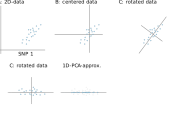
\includegraphics[width=\textwidth]{pca_explanation.png}
		\caption{Basic Idea of PCA from 2D to 1D representation. A: Allele frequencies from different populations (blue dots) at two SNPs. A PCA is performed by centering the data (B), and rotating it (B) such that the first PC explains the majority of variation in the data, and the second PC is orthognal to the first, and explains the residual. A lower-dimensional approximation (in this case 1D) can be achieved by just keeping the first PC (E); which can be translated back to the original data space by inverting the rotation and centering (F).}
		\label{fig:pca_explanation}
	\end{figure}
	
	There are several algorithms that are used to calculate a PCA in practice, the most common one relies on a singular value decomposition. In this approach, we first mean-center $\MX$ to obtain the centered matrix $\MY$
	\begin{equation}
	y_{il} = x_{il} - \mu_l
	\end{equation}
	where $\mu_l$ is the mean allele frequency at the $l$-th locus.
	
	PCA can then be written as
	
	\begin{equation}
	\MY = \MC\MX = (\mathbf{U} \MSINGULAR) \mathbf{V}^T = \MP\ML\text{,}
	\end{equation}
	
	where $\MC = \mathbf{I} -\frac{1}{n}\mathbf{1}$ is a centering matrix that subtracts row means, with $\mathbf{I}, \mathbf{1}$  the identity matrix and a matrix of ones, respectively. The orthogonal matrix of principal components $\MP=\mathbf{U}\MSINGULAR$ has size $n \times n$ and is used to reveal population structure. The loadings $\ML=\mathbf{V}^T$ are an orthonormal matrix of size $n \times k$, its rows give the contribution of each SNP to each PC, it is often useful to look for outliers that might be indicative of selection \cite[e.g][]{francois2010}.
	
	In many  implementations \citep[e.g]{patterson2006}, SNPs are weighted by the inverse of their standard deviation. As these weights makes little difference in practice and obfuscate the connection to $F$-statistics, I will for now assume that SNPs are unweighted, and defer discussion of weighting to a later section.
	

	
\subsection{Introduction to $F$-statistics}
From a modeling perspective, $F$-statistics have been primarily motivated by trees and admixture graphs \citep{patterson2012}, but can be calculated for arbitrary population genetics models for which expected pairwise coalescence times are known \citep{peter2016}. 

They are based on the squared Euclidean distance $F_2$ used as a tree metric, and the 
\begin{subequations}
	\begin{align}
	F_2(X_1, X_2) &= \sum_i^k (x_{1i} - x_{2i})^2 = 2\mathbb{E}T_{12} - \mathbb{E}T_{11} - \mathbb{E}T_{22} &=& \normsq{X_1 - X_2}\\
	F_3(X_1; X_2, X_3) &= \sum_i^k (x_{1i} - x_{2i})(x_{1i} - x_{3i}) &=& \langle X_1 - X_2, X_1 - X_3 \rangle\\
	F_4(X_1 X_2; X_3, X_4) &= \sum_i^k (x_{1i} - x_{2i})(x_{3i} - x_{4i}) &=& \langle X_1 - X_2, X_3 - X_4 \rangle,
	\end{align}
\end{subequations}
where the $X_i$ are rows of $\MX$ that represent all loci of population $i$, and the $T_{ij}$ denote the pairwise coalescence time of two sampled individuals from population $i$ and $j$.

Here, much of the focus is not on interpreting these $F$-statistics in terms of model, but in \emph{data space}. For this, we interpret $F$-statistics as inner products on $\mathbb{R}^L$, and the norm $\norm{\cdot}$ and inner product $\langle\cdot, \cdot \rangle$ notation are used to make the connection to Euclidean geometry more explicit \citep[see][for a thorough introduction to this interpretation]{oteo-garcia2021}.

\subsection{PCA from $F$-statistics}
Despite their different motivation, $F$-statistics and PCA are closely related through a procedure called multidimensional scaling (MDS). For MDS, we consider a matrix 	$\MF, f_{ij} = F_2(X_i, X_j)$ of pairwise $F_2$-statistics. Then, the matrix of principal components $\MP$ can be obtained by performing an eigendecomposition of the double-centered $\MF$-matrix  \cite{gower1966}:
\begin{equation}
\MP\MP^T = -\frac{1}{2} \MC \MF\MC \text{.}
\end{equation}


\subsection{$F$-statistics in PCA-space}
The $F$-statistics can be thought of as inner products in the Euclidean allele-frequency space. By performing a PCA, we just translate and rotate our data, but the dot products is invariant under both these operations. Hence, neither mean-centering (a translation) nor PCA (a rotation) will change $F_2$. What this means is that we are free to calculate $F_2$ either on the uncentered data $\MX$, the centered data $\MY$ or the principal components $\MP$. Formally,

\begin{align}
F_2(X_i, X_j) &=&  \sum_{l=1}^L \big( x_{il} -x_{jl}\big)^2 &&\nonumber\\ 
 &=& \sum_{l=1}^L \big( (x_{il} - \mu_l) -(x_{jl} -\mu_l)\big)^2  &=& F_2(Y_i, Y_j) \nonumber\\
 &=& \sum_k (P_{ik} - P_{jk})^2  &=& F_2(P_i, P_j) \text{,}
\end{align}
A detailed derivation of this is given in Appendix \ref{appendix:fonpc}.
As $F_3$ and $F_4$ can be written as sums of $F_2$-terms \citep{reich2009}, analogous relations apply.

\subsection{Geometric representation of $F$-statistics in PC-space}
The transformation derived in the previous section allows us to consider the geometry of $F$-statistics in the rotated PCA-space. The relationships we will discuss formally only hold if we use all $n-1$ PCs. However, the appeal of PCA is that frequently, only a very small number $K \ll n$ of PCS contain most information that is relevant for population structure.

Here, we start by discussing 2-dimensional spaces. This is useful for two reasons: for one, the geometry is simpler and we can think of circles as opposed to $n$-balls and other high-dimensional geometric objects. Second, in many applications it is argued that a 2-dimensional approximation is sufficient to explain the major components of population structure \cite[e.g.][]{novembre2008}. In this case, the results here will hold under the same approximation assumptions in low-dimensional PCs; if they differ substantially from each other, it is likely that not sufficiently many PCs were considered.


\subsubsection{$F_2$ in 2D PC-space}
The $F_2$-statistic is an estimate of the squared Euclidean distance is the easiest to understand, it corresponds directly to the squared distance in PCA-space. This matches our intuition that closely related populations (which have low $F_2$) will be close to each other on a PCA-plot.


\subsubsection{$F_3$ and circles}
A common application of $F_3$-statistics is to test for admixture; we say that population $X_x$ is admixed from sources $X_1$ and $X_2$ if $F_3(X_x; X_1, X_2) < 0$. This motivates the following question: given two source populations $X_1$, $X_2$, where would we expect the admixed population $X_x$ on a PCA plot? Since the allele frequencies of $X_x$ are intermediate between $X_1$ and $X_2$, we would expect it to lie between these two populations \cite{brisbin2012, mcvean2009}, but we can make this notion more precise:

\begin{eqnarray}
2 F_3(X_x; X_1, X_2) &=& \langle  X_x - X_1, X_x - X_2 \rangle \nonumber\\
      &=& \normsq{X_x - X_1} + \normsq{X_x - X_2}  - \normsq{X_1 - X_2} \nonumber\\
      &<&0
\end{eqnarray}
By the Pythagorean theorem, $F_3 = 0 $ iff $X_1, X_2$ and $X_x$ form a right-angled triangle. Hence, on a 2D-PCA-plot, the region where $F_3$ is zero is the circle with diameter $\overline{X_1X_2}$ (Figure \ref{fig:fstats_theory}B). If $X_3$ lies inside this circle, the angle is obtuse and $F_3$ is negative, otherwise it will be positive. If we consider all PCs, the circle is replaced by a $n$-ball with diameter $\overline{X_1X_2}$, but otherwise the reasoning is exactly the same. In this case, not all populations inside a circle on a 2D-plot will have negative $F_3$, as they may be outside the $n$-ball in another dimension. However, all populations that map outside the circle on any PC are guaranteed to have a positive associated $F_3$-statistic.


Similarly, if we fix the admixed population $X_x$ and one source $X_1$, we may ask where on a 2D-PCA-plot $X_2$ would lie if $F_3(X_x; X_1, X_2) < 0$. This space is similarly defined by all the points for which the angle between the line segments $\overline{X_1X_x}$ and $\overline{X_2 X_x}$ is obtuse (Figure \ref{fig:fstats_theory}C). In this case

\begin{figure}[!ht]
	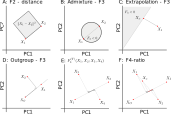
\includegraphics[width=\textwidth]{dummy_pca.png}
	\caption{\textbf{Geometric representation of $F$-statistics on 2D-PCA-plot.} A: $F_2$ represents the squared Euclidean distance between two points in PC-space. B: Admixture-$F_3(X_x; X_1, X_2)$ is negative if $X_x$ lies in the circle specified by the diameter $X_2-X_1$}. C: $F_3(X_x; X_1, X_2)$ is negative given $X_1, X_x$ if $X_2$ is in the gray space.  D: Outgroup-$F_3$ reflects the projection of $X_2 - X_O$ on $X_1 - X_O$. E: $F_4$ is the projection of $X_3 - X_4$ on $X_1-X_2$. F: If $X_x$ is admixed between $X_1$ and $X_2$, the admixture proportions will be projected.
	\label{fig:fstats_theory}
\end{figure}

\subsubsection{$F_4$ and right angles}
The inner-product-interpretation of $F_4$ is similar to that of $F_3$, with the change that the two vectors we consider do not involve the same population. However, a finding of $F_4(X_1, X_2; X_3, X_4) = \langle X_1 - X_2, X_3 - X4 \rangle = 0$ similarly implies that the two vectors are orthogonal, and a non-zero value reflects the projection of one vector on the other.

\subsubsection{$F_4$-ratio}
\begin{eqnarray}
\frac{F_4(X_I, X_O; X_X, X_1)}{F_4(X_I, X_O; X_2, X_1)} &=& \frac{\norm{X_I-X_O}\norm{X_X-X_1}\cos(\alpha)}{\norm{X_I-X_O}\norm{X_2-X_1}\cos(\beta)}\nonumber\\
&=&\frac{\norm{X_X-X_1}\cos(\alpha)}{\norm{X_2-X_1}\cos(\beta)}\nonumber\\
&=& \frac{\norm{X_X' - X_1'}}{\norm{X_2' - X_1'}}
\end{eqnarray}
where $\alpha$ and $\beta$ are the angles between vectors, and $X_i'$ is the projection of $X_i$ on $X_I-X_O$.

Conjecture: Thus, we are measuring the distances between the admixing populations on the projected on the axis between $X_I$ and $X_O$. This ought to be valid only if $\langle X_1 - X_1', X_2 - X_2' \rangle$ are orthogonal to each other, and to $X_OX_I$, i.e.
$F_4(X_1, X_1', X_2, X_2') = 0$
 
	
\subsection{Higher-Dimensional Spaces}


\section{Results}
\begin{figure}[!ht]
	\includegraphics[width=\textwidth]{figures/fig_f3_data.pdf}
	\caption{\textbf{PCA and $F_3$-statistics} A: PCA of Western Eurasian data; the circle denotes the region for which $F_3(X; \text{Basque}, \text{Turkish})$ may be negative. Populations for which $F_3$ is negative are colored in red. B, E: $F_3$ approximated with two (blue) and ten (red) PCs versus the full spectrum. C,F: Contributions of PCs 1-10 to each $F_3$-statistic. D: PCA of World data set, color indicates value of $F_3(\text{Mbuti}; \text{Mozabite}, X)$. The black line shows the projection axis Mbuti-Mozabite, the gray lines indicates the projected position of each population. }
	\label{fig:f3}
\end{figure}

\begin{figure}[!ht]
	
\includegraphics[width=\textwidth]{figures/fig_f4_data.pdf}	
	\caption{\textbf{PCA and $F_4$-statistics} A: Spectrum of select $F_4$-statistics in World data set. B: Projection angle representation of $F_4(X, Sardinian; Mozabite, Yoruba)$ (red) and approximations using two (blue) and ten (green) PCs. C: Spectrum of select $F-4$-statistics in Westeurasian data set. D: Scatterplot of $F_4$-projection on Finnish-Canary Islanders axis and residual PC1.
		E: $F_4(X, \text{French}, \text{Finnish}, \text{Canary Islander})$ vs. prediction using two (blue) and ten(red) PCs. F: Percent variance explained for the projection of panel D and the first nine residual PCs.
	}
	\label{fig:f4}
\end{figure}

\section{Trees and admixture graphs in PCA-space}
\subsection{Trees}
Evolutionary trees are fundamental in phylogenetic analyses, as they, on a large, scale, approximate how taxa diversify. Within a species, applying trees is also very common, but more problematic as populations frequently do not evolve as discrete lineages; instead, they admix and diversify as much more continuous processes. This is largely due to the time-scales involved, speciation events that give rise to trees might often be similarly messy, but from a distance of millions of years these issues might disappear. 

Thus, when estimating trees from population genetic data, we must be very careful about whether the data is actually consistent with a tree, or belongs to some wider class of model.


Trees can be thought of as a collection of orthogonal dimensions; as drift on each branch is independent from every other branch. Thus, each sample is only 
\begin{enumerate}
	\item Trees
	\item Admixture Graphs
	\item Treelets
	\item simple trees, admixture graph
\end{enumerate}


\section{Technical considerations}
	\subsection{SNP weighting}
	It is clear that weighting SNP will have some effect on the resulting PCAs. Upweighting rare variants e.g. will emphasis recent events, as rare variance in the sample are more likely to be recent.
	
	
	\subsection{Missing data}
	
	\subsection{$F_2$ error}
	In most $F$-statistics applications, $F_2$ is \emph{estimated} using the minimum-variance unbiased estimator \citep{reich2009}
	\begin{subequations}

	\begin{equation}
	f_2(X_1, X_2) = \frac{1}{L}\sum_l (x_{l1} - x_{l2})^2 - \frac{1}{L}\sum_l\frac{x_{l1} (1-x_{l1})}{n_{l1}-1} - 
	\frac{1}{L}\sum_l\frac{x_{l2} (1-x_{l2})}{n_{l2}-1} - 
	\end{equation}
	in contrast, as shown above, PCA can be thought as a decomposition of a matrix of uncorrected $F_2$-statistics:
	\begin{equation}
	F_2(X_1, X_2) = \frac{1}{L}\sum_l(x_{l1} - x_{l2})^2
	\end{equation}
	\end{subequations}

	This leads to some issues, for example trying to perform a PCA on the matrix of $f_2$-values is not positive semidefinite, and so some principal components may be imaginary. One possible resolution is probabilistic PCA \citep[e.g.][]{engelhardt2010,agrawal2020}.
	
	\begin{align}
	    y_{ij} | \MP_{ij}, \epsilon_i &= (\MP\ML)_{ij} + \epsilon_{ij}\nonumber\\
	    x_i & \sim N(0, \mathbf{I}) \nonumber\\
	    \epsilon_i &\sim N(0, \sigma^2 \mathbf{I})\nonumber
	\end{align}
	
	\subsection{qpADM}
	In \cite{haak2015}, qpADM, a procedure to estimate admixture proportions has been proposed. qpADM aims to solve equations of the form
	
	\begin{align}
	\langle P_X - A, B -C \rangle &= \sum_i  \alpha_i\langle R_i - A, B - C \rangle \nonumber\\
	&= \left\langle \sum_i  \alpha_i R_i - A, B - C \right\rangle
	\end{align}
	
	
	\subsection{What is a dimension?}
	In both the PCA and $F$-statistic framework, a population at  a particular point in time can be thought of as a single point in allele-frequency space, given by the $k$-dimensional vector $v_0$ of allele frequencies at the $k$ SNPs in that population. If this population evolves for some time in isolation, allele frequencies will change due to genetic drift from $v_0$ to some other point $v_1$. Likewise, a second population with frequency $w_0$ will move to $w_1$. Crucially, if these populations do not interact, the changes in allele frequency, $v_1 - v_0$ and $w_1 - w_0$ will be uncorrelated \cite{patterson2012}. Thus, if we have two populations that descend from the same ancestral population in isolation, they can be thought of as evolving along orthognal dimensions from the same point. This argument is at the foundation of F-statistics.
	
	
	\section{outtakes}
	PCA from $\MX$
	\begin{equation}
	\MK = \MY \MY^T = \MC\MX\MX^T \MC = \MP\MP^T
	\end{equation}

\section{Discussion}
The fa



\appendix
\section{Derivation}\label{appendix:fonpc}
\begin{eqnarray}
F_2(X_i, X_j) &=& \sum_{l=1}^L \big( (x_{il} - \mu_l) -(x_{jl} -\mu_l)\big)^2 = F_2(Y_i, Y_j)\nonumber\\
&=& \sum_{l=1}^L \big( \sum_k L_{kl}P_{ik} - \sum_kL_{kl}P_{kj}\big)^2\nonumber\\
&=& \sum_{l=1}^L \left( \sum_k L_{kl} (P_{ik} -P_{jk}) \right)^2\nonumber\\
&=& \sum_{l=1}^L \left( \sum_k L_{kl}^2 (P_{ik} -P_{jk})^2 + 2\sum_{k\neq k'} L_{kl}L_{k'l}(P_{ik} - P_{jk'})^2 \right)\nonumber\\
&=& \sum_k \underbrace{\left(\sum_{l=1}^L L_{kl}^2\right)}_1 (P_{ik} -P_{jk})^2 + \sum_{k\neq k'}\underbrace{\left(\sum_{l=1}^L L_{kl}L_{k'l}\right)}_{0} (P_{ik} - P_{jk'})^2\nonumber\\
&=& \sum_k (P_{ik} - P_{jk})^2
\end{eqnarray}

In summary, the first row shows that $F_2$ on the centered data will give the same results (as distances are invariant to translations), in the second row we apply the PC-decomposition. The third row is obtained from factoring out $L_{lk}$. Row four is obtained by multiplying out the sum inside the square term for a particular $l$. We have $k$ terms when for $\binom{k}{2}$ terms for different $k$'s.  Row five is obtained by expanding the outer sum and grouping terms by $k$.The final line is obtained by recognizing that $\ML$ is an orthonormal basis; where dot products of different vectors have lengths zero.

Note that if we estimate $F_2$, unbiased estimators are obtained by subtracting the population-heterozygosities $H_i, H_j$ from the statistic. As these are scalars, they do not change above calculation.
\bibliography{main}

\end{document}
